\documentclass[12pt,a4paper]{book}
\raggedbottom

\usepackage{ugmath}
\usepackage{float}
\usepackage{placeins}
\usepackage[labelfont=bf,labelsep=space]{caption}
\usepackage{pdfpages}
\usepackage{graphicx}
\begin{document}
    

    \thispagestyle{empty}
    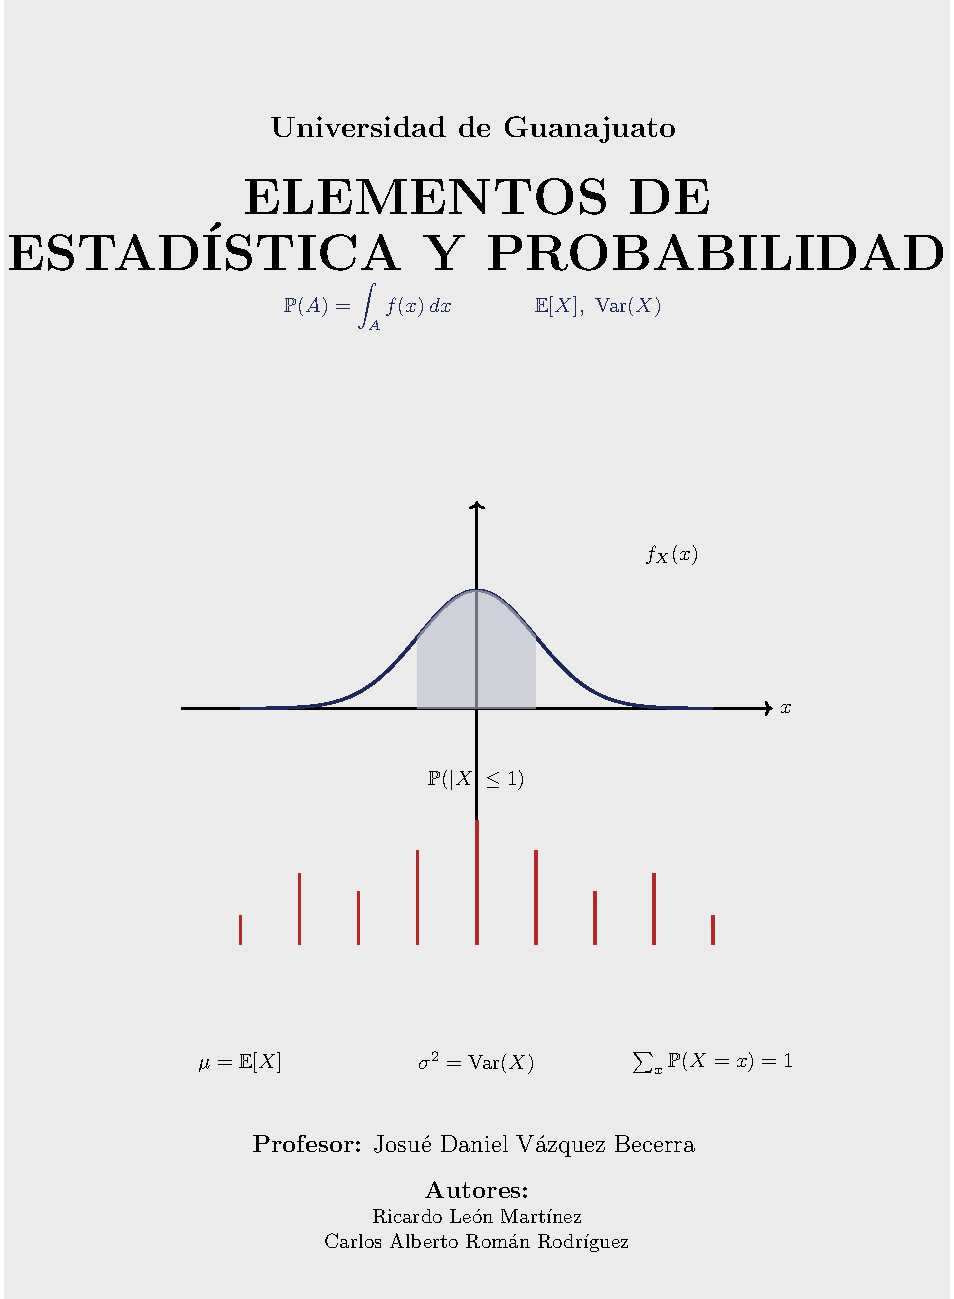
\includepdf[pages=1]{probita.pdf}
    

    \setcounter{page}{1}
    \tableofcontents
    \clearpage

    \chapter{Teoría de conjuntos y combinatoria}

    \section{Combinatoria}

    La \textbf{Combinatoria} es una rama de las matemáticas que se dedica al estudio de las técnicas y métodos para contar configuraciones y disposiciones de objetos. Además de su interés intrínseco, la combinatoria tiene aplicaciones de gran relevancia en diversas áreas, especialmente en la \textbf{Probabilidad}, donde proporciona herramientas fundamentales para el calculo y análisis para el cálculo y análisis de eventos aleatorios.

    \subsection{Dos Principios Básicos}

    \textbf{Problemas Básicos de Combinatoria}\\
    Comenzaremos analizando algunos problemas sencillos que ilustran los principios fundamentales de la combinatoria.

    \begin{mdframed}[style=mdgraybox,frametitle={Problema 1: Combinación de prendas}]
        En una tienda hay cinco modelos de camisas y tres modelos de pantalones. ¿Cuántos conjuntos distintos de patalón y camisa se pueden comprar?
    \end{mdframed}

    \begin{solucion}
        La camisa puede elegirse de 5 maneras distintas. Para cada camisa selccionada, hay 3 opciones de pantalón. Por lo tanto, el número total de conjuntos distintos es:
        \begin{equation*}
            5\times3=15.
        \end{equation*}
    \end{solucion}

    \begin{mdframed}[style=mdgraybox,frametitle={Problema 2: Rutas entre ciudades}]
        Las ciudades $A,B$y $C$ están conectadas como se muestra en la Figura 1.1. Hay seis caminos de $A$ a $B$ y cuatro caminos de $B$ a $C$. ¿De cuántas maneras se puede viajar de $A$ a $C$?
        \begin{figure}[H]
            \centering
            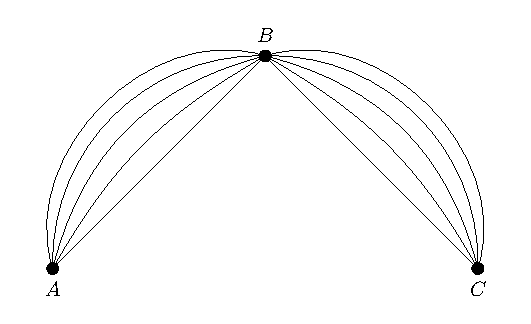
\includegraphics[width=0.7\textwidth]{camino.pdf}
            \caption{Conexiones entre las ciudades $A$, $B$ y $C$.}
            \label{fig:conexiones}
        \end{figure}
    \end{mdframed}

    \begin{solucion}
        Para cada camino entre $A$ y $B$, hay 4 opciones para continuar de $B$ a $C$.
        Como hay 6 caminos entre $A$ y $B$, el número total de rutas de $A$ a $C$ es:
        \begin{equation*}
            6\times4=24.
        \end{equation*}
    \end{solucion}

    \begin{mdframed}[style=mdgraybox,frametitle={Problema 3: Producto cartesiano}]
        Sean $A=\{a_{1},a_{2},\dots,a_{k}\}$ un conjunto con $k$ elementos y $B=\{b_{1},b_{2},\dots,b_{n}\}$ un conjunto con $n$ elementos. ¿Cuantos elementos tiene el producto cartesiano $A\times B$?
    \end{mdframed}

    \begin{solucion}
        El producto cartesiano $A\times B$ consiste en todos los pares ordenados $(a,b)$, donde $a\in A$ y $b\in B$. Para cada uno de los $k$ elementos de $A$, hay $n$ opciones en $B$ para formar un par. Por lo tanto, el número total de pares ordenados es
        \begin{equation*}
            k\times n.
        \end{equation*}
    \end{solucion}
    Estos problemas ilustran el principio básico de la multiplicación en combinatoria, que es fundamental para contar configuraciones y disposiciones.\\
    \textbf{Principio de Multiplicación}\\
    El resultado general puede enunciarse de la siguiente manera
    
    \begin{mdframed}[style=mdpinkbox,frametitle={Principio Multiplicativo}]
        Si tenemos dos conjuntos, uno con $k$ elementos y otro con $n$ elementos, y queremos selccionar un elemento del primero y otro del segundo, esto puede hacerse de $k\times n$ maneras distintas.
    \end{mdframed}

    Este principio puede aplicarse de manera reiterada para resolver problemas más complejos, como se muestra en los siguientes ejemplos.

    \begin{mdframed}[style=mdgraybox,frametitle={Problema 4: Combinaciones de prendas y zapatos}]
        En la tienda del \textbf{Problema 1}, además de las camisas y pantalones, hay cuatro modelos distintos de zapatos. ¿De cuántas maneras podemos escoger un conjunto que incluya una camisa, un pantalón y un par de zapatos?
    \end{mdframed}

    \begin{solucion}
        Del \textbf{Problema 1}, sabemos que hay 15 conjuntos posibles de camisa y pantalón. Para cada uno de estos conjuntos, hay 4 opciones de zapatos. Por lo tanto, el número total de conjutnos de camisa, pantalón y zapatos es
        \begin{equation*}
            15\times 4=60
        \end{equation*}
    \end{solucion}

    \begin{mdframed}[style=mdgraybox,frametitle={Problema 5: Selección de objetos de diferentes tipos}]
        Una costurera tiene tres botones, cinco agujas y ocho tipos de hilo. ¿De cuántas maneras puede escoger un objeto de cada tipo?
    \end{mdframed}

    \begin{solucion}
        Para los tres botones, hay 3 opciones. Para las agujas, hay 5 opciones. Para los hilos, hay 8 opciones. Aplicando el principio de multiplicación, el número total de maneras de escoger un objeto de cada tipo es
        \begin{equation*}
            3\times 5\times 8=120.
        \end{equation*}
    \end{solucion}

    Estos ejemplos ilustran cómo el principio de multiplicación puede extenderse a situaciones con más de dos conjuntos, permitiendo contar configuraciones complejas de manera sistemática.\\
    \textbf{Problemas Adicionales de Combinatoria}\\
    A continuación, exploraremos otro tipo de problemas que amplían la aplicación del principio de multiplicación y la suma en combinatoria.

    \begin{mdframed}[style=mdgraybox,frametitle={Problema 6: Rutas entre ciudades con una cuerta ciudad}]
        Consideremos las ciudades $A,B,C$ y una cuarta ciudad $D$, conectadas como se muestra en la figura 1.2. ¿De cuántas maneras podemos viajar de $A$ a $C$?
        \begin{figure}[H]
            \centering
            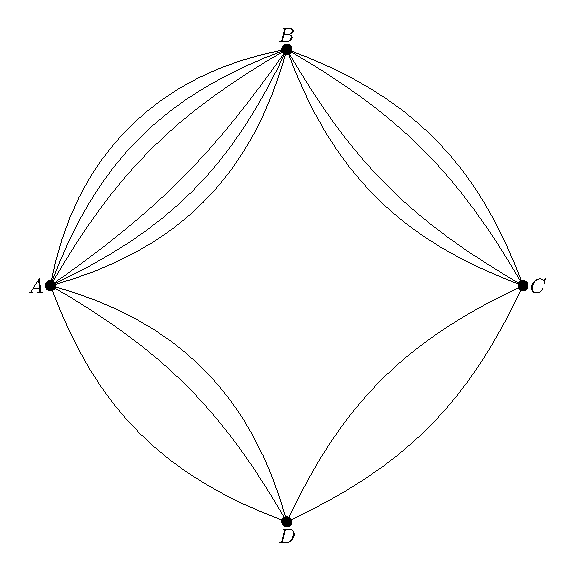
\includegraphics[width=0.7\textwidth]{camino2.pdf}
            \caption{Conexiones entre las ciudades $A$, $B$ y $C$.}
            \label{fig:conexiones2}
        \end{figure}
    \end{mdframed}

    \begin{solucion}
        Podemos viajar de $A$ a $C$ pasando por $B$ o por $D$. Por el \textbf{Problema 2}, sabemos que hay 24 maneras de ir $A$ a $C$ pasando por $B$. Aplicando el principio de multiplicación, hay $3\times2=6$ maneras de ir de $A$ a $C$ pasando por $D$. Por lo tanto, el número total de rutas de $A$ a $C$ es
        \begin{equation*}
            24+6=30.
        \end{equation*}
    \end{solucion}

    \begin{mdframed}[style=mdgraybox,frametitle={Problema 7: Elección de pantalones en dos tiendas}]
        Una persona visita dos tiendas con la intención de comprar un pantalón. En la primer tienda hay seis modelos diferentes, y para cada modelo hay tres colores disponibles. En la segunda tienda hay diez modelos, y para cada modelo hay cuatro colores. ¿Entre cuántos pantalones tiene que escoger la persona?
    \end{mdframed}

    \begin{solucion}
        En la primero tienda, el número total de pantalones es
        \begin{equation*}
            6\times3=18.
        \end{equation*}
        En la segunda tienda, el número total de pantalones es
        \begin{equation*}
            10\times 4=40.
        \end{equation*}
        Para obtener el total de pantalones disponibles, sumamos las opciones de ambas tiendas
        \begin{equation*}
            18+40=58.
        \end{equation*}
    \end{solucion}
    
    Estos problemas ilustran cómo combinar el principio de multiplicación y la suma para resolver situaciones mas complejas en combinatoria.\\
    \textbf{Principio Aditivo}\\
    En los problemas anteriores, observamos que existen situaciones excluyentes:
    \begin{itemize}
        \item Para viajar de $A$ a $C$, se puede pasar por $B$ o $D$, pero no por ambos.
        \item Para comprar un pantalón, se puede elegir entre la primera tienda o la segunda, pero no en ambas.
    \end{itemize}

    En estos casos, el número total de soluciones se obtiene sumando las soluciones de cada alternativa. Este resultado se formalizan en el siguiente principio:

    \begin{mdframed}[style=mdpinkbox,frametitle={Principio Aditivo}]
        Si una situación puede ocurrir de $k$ maneras distintas y una segunda situación, excluyente de la primera, puede ocurrir de $n$ maneras distintas, entonces existe $k+n$ maneras en las que puede ocurrir la primera o la segunda situación.
    \end{mdframed}

    Este principio también puede aplicarse de manera reiterada, como se ilustra en los siguientes problemas.

    \begin{mdframed}[style=mdgraybox,frametitle={Problema 8: Compra de dos objetos distintos}]
        En una tienda hay cinco modelos de pantalón, ocho de camisa y cuatro de zapatos. ¿Cuántas maneras hay de comprar dos objetos de tipos distintos?
    \end{mdframed}

    \begin{solucion}
        Hay tres casos posibles
        \begin{enumerate}
            \item Comprar pantalón y camisa: $5\times8=40$ maneras.
            \item Comprar pantalón y zapatos: $5\times4=20$ maneras.
            \item Comprar camisa y zapatos: $8\times3=32$ maneras.
        \end{enumerate}
        Aplicando el principio aditivo, el número totasl de maneras es
        \begin{equation*}
            40+20+32=92.
        \end{equation*}
    \end{solucion}

    \begin{mdframed}[style=mdgraybox,frametitle={Problema 9: Números de hasta tres cifras}]
        ¿Cuantas números de, a lo sumo, tres cifras se pueden formar con los dígitos 3,4,7 y 8?
    \end{mdframed}

    \begin{solucion}
        Los números pueden tener una, dos o tres cifras. Analizamos cada caso por separado y luego sumamos los resultados:
        \begin{itemize}
            \item \textbf{Números de una cifra:} Hay 4 opciones (3,4,7,8).
            \item \textbf{Números de dos cifras:} La primera y la segunda cifra pueden ser cualquiera de los cuatro dígitos. Por lo tanto, hay $4\times4=16$ números.
            \item \textbf{Números de tres cifras:} Cada una de las tres cifras puede ser cualquiera de los cuatro dígitos. Así, hay $4\times4\times4=64$ números.
        \end{itemize}
        Aplicando el principio aditivo, el número total de números de hasta tres cifras es
        \begin{equation*}
            4+16+64=84.
        \end{equation*}
    \end{solucion}

    Estos problemas demuestran cómo el principio aditivo se combina con el principio multiplicativo para resolver situaciones más complejas en combinatoria.

    \subsection{Número de subconjuntos de un conjunto finito}

    Sea $C=\{c_{1},c_{2},\dots,c_{n}\}$ un conjunto finito con $n$ elementos. Denotamos por
    $\mathcal{P}(C)$ el conjunto de partes de $C$, es decir, la familia de todos sus subconjuntos.

    \textbf{Ejemplo}\\
    Para $C=\{c_{1},c_{2},c_{3}\},\mathcal{P}(C)$ incluye:
    \begin{equation*}
        \emptyset,\{c_{1}\},\{c_{2}\},\{c_{3}\},\{c_{1},c_{2}\},\{c_{1},c_{3}\},\{c_{2},c_{3}\},\{c_{1},c_{2},c_{3}\}.
    \end{equation*}
    En total, $\mathcal{P}(C)$ tiene 8 subconjuntos.

    \textbf{Método general}\\
    Para calcular $\abs{\mathcal{P}(C)}$, construimos subconjuntos asignado a cada elemento,
    $c_{i}$ un 1 (si se incluye) o un 0 (si no se incluye). Esto equivale a generar todas las $n$-tuplas de ceros y unos:
    \begin{equation*}
        A_{n}=\{(a_{1},a_{2},\dots,a_{n}):a_{i}\in\{0,1\}\}
    \end{equation*}
    Cada $n$-tupla corresponde a un subconjunto único. Por ejemplo: $\{c_{1}\}$ se asocia con (1,0,0). $\{c_{2},c_{3}\}$ se asocia con (0,1,1).

    \textbf{Cálculo del número de subconjuntos}\\
    Para calcular $\abs{A_{n}}$, observamos lo siguiente:
    \begin{itemize}
        \item Para $n=1$, hay 2 1-tuplas: (0) y (1).
        \item Para $n=2$, hay 4 2-tuplas: (0,0),(0,1),(1,0), y (1,1).
        \item Para $n=3$, hay 8 3-tuplas:
        \begin{align*}
            (0,0,0),(0,1,0),(1,0,0),(1,1,0),\\
            (0,0,1),(0,1,1),(1,0,1),(1,1,1).
        \end{align*}
    \end{itemize}
    En general, para $n\geq2$, se cumple que:
    \begin{align*}
        \abs{A_{n}}=2\cdot(\abs{A_{n-1}}),
    \end{align*}
    donde $\abs{A_{n}}$ representa el número de $n$-tuplas. Mediante un argumento inductivo,
    concluimos que:
    \begin{equation*}
        \abs{A_{n}}=2^{n}.
    \end{equation*}
    Por tanto, el número de subconjuntos de $C$ es:
    \begin{equation*}
        \abs{\mathcal{P}(C)}=2^{n}.
    \end{equation*}

    \subsection{Variaciones con Repetición}

    
    En esta sección, exploraremos problemas que involucran la formación de secuencias o combinaciones donde los elementos pueden repetirse. A continuación, presentamos algunos ejemplos ilustrativos.

    \begin{mdframed}[style=mdgraybox,frametitle={Problema 10: Lanzamiento de una moneda}]
        Se lanza una moneda tres veces. ¿Cuántas sucesiones distintas de águilas y soles se pueden obtener?
    \end{mdframed}

    \begin{solucion}
        En cada lanzamiento hay dos resultados posibles: águila o sol. Para los tres lanzamientos, el número total de sucesiones distintas es
        \begin{equation*}
            2\times2\times2=2^{3}=8.
        \end{equation*}
    \end{solucion}

    \begin{mdframed}[style=mdgraybox, frametitle={Problema 11: Números de cuatros cifras impares}]
        ¿Cuántos números de exactamente cuatro cifras se pueden formar usando solo dígitos impares?
    \end{mdframed}

    \begin{solucion}
        Los dígitos impares son 1,3,5,7 y 9, es decir, 5 opciones. Cada una de las cuatro cifras (unidades, decenas, centenas y unidades de mil) puede ser cualquiera de estos dígitos. Por lo tanto, el número total de números de cuatro cifras impares es:
        \begin{equation*}
            5\times5\times5\times5=5^{4}=625.
        \end{equation*}
    \end{solucion}

    \begin{mdframed}[style=mdgraybox,frametitle={Problema 12: Palabras de tres letras}]
        ¿Cuántas palabras de tres letras (con o sin sentido) pueden formarse con las letras de la palabra \textbf{AZUL}?
    \end{mdframed}

    \begin{solucion}
        La palabra \textbf{AZUL} tiene cuatro letras distintas: $A,Z,U,L$. Para cada una de las tres posiciones en la palabra, hay 4 opciones. Por lo tanto, el número total de palabras de tres letras es:
        \begin{equation*}
            4\times4\times4=4^{3}=64.
        \end{equation*}
    \end{solucion}
    
    Estos problemas ilustran el concepto de \textbf{variaciones con repetición}, donde cada posición en la secuencia puede ocuparse con cualquier elemento del conjunto dado, permitiendo repeticiones.\\

    {\large \textbf{Variaciones con Repetición}}

    Consideremos un conjunto $C=\{c_{1},c_{2},\dots,c_{m}\}$ con $m$ elementos. Nos interesa estudiar el conjunto de $n-$tuplas (o vectores de dimensión $n$) que pueden formarse con los elementos de $C$, permitiendo repeticiones. Este conjunto se denota como:
    \begin{equation*}
        X_{n}=\{(c_{i_{1}},c_{i_{2}})\}
    \end{equation*}
    \textbf{Ejemplos}\\
    1. Si $C=\{0,1\}$, entonces $X_{n}$ corresponde al conjunto $A_{n}$ de $n-$tuplas de ceros y unos.\\
    2. Si $C=\{0,1,2\}$ y $n=3$, el conjunto $X_{n}$ está formado por las siguientes ternas:
    \begin{equation*}
        \begin{array}{c}
            (0, 0, 0), (0, 0, 1), (0, 0, 2), (0, 1, 0), (0, 1, 1), (0, 1, 2), (0, 2, 0), (0, 2, 1), (0, 2, 2), \\
            (1, 0, 0), (1, 0, 1), (1, 0, 2), (1, 1, 0), (1, 1, 1), (1, 1, 2), (1, 2, 0), (1, 2, 1), (1, 2, 2), \\
            (2, 0, 0), (2, 0, 1), (2, 0, 2), (2, 1, 0), (2, 1, 1), (2, 1, 2), (2, 2, 0), (2, 2, 1), (2, 2, 2).
        \end{array}
    \end{equation*}

    \textbf{Observación sobre el orden}\\
    A diferencia de los subconjuntos, el orden de las componentes en una $n-$tupla es determinante. Por ejemplo, la $2-$tupla $(c_{1},c_{2})$ es distinta de $(c_{2},c_{1})$, a menos que $c_{1}=c_{2}$. Esto resalta la importancia del orden en las variaciones con repetición.

    {\large \textbf{Cálculo del número de variaciones con repetición}}

    Para calcular el número de elementos de $X_{n}$, conocido como \textbf{variaciones con repetición} de $m$ elementos tomados de $n$ en $n$, seguimos un razonamiento similar al utilizado en la sección anterior para contar $n-$tuplas de ceros y unos. La diferencia es que ahora las $n-$tuplas se forman con los $m$ elementos de $C$. Repitiendo el mismo argumento, obtenemos:
    \begin{equation*}
        \abs{X_{n}}=m^{n}
    \end{equation*}

    \begin{mdframed}[style=mdgraybox,frametitle={Problema 13: Lanzamiento de un dado}]
        Si lanzamos un dado cuatro veces, ¿cuantos resultados posibles hay?
    \end{mdframed}

    \begin{solucion}
        Para cada lanzamiento, hay 6 resultados posibles (los números del 1 al 6). Como el dado se lanza 4 veces, el número total de resultados posibles es:
        \begin{equation*}
            6^{4}=1296
        \end{equation*}
    \end{solucion}

    En la notación anterior, $C=\{1,2,3,4,5,6\}$, $m=6$ y $n=4$.

    \begin{mdframed}[style=mdgraybox,frametitle={Problema 14: Pintura de casas}]
        En una cuadra hay cinco casas. Hay tres colores disponibles para pintar cada una de ellas. ¿De cuántas maneras se puede pintar el conjunto de las cinco casas?
    \end{mdframed}

    \begin{solucion}
        Para cada casa, hay 3 opciones de color. Como hay 5 casas, el número total de maneras de pintarlas es:
        \begin{equation*}
            3^{5}=243.
        \end{equation*}
    \end{solucion}
    Estos problemas ilustran cómo el concepto de variaciones con repetición se aplica en situaciones prácticas, permitiendo calcular el número de configuraciones posibles cuando los elementos pueden repetirse.

    \subsection{Variaciones sin repeticiones}

    Ahora consideraremos problemas en los que la selección de elementos es ordenada y sin repetición. Esto significa que, una vez seleccionado un elemento, no puede volver a ser elegido.

    \begin{mdframed}[style=mdgraybox,frametitle={Problema 15: Selección de capitán y suplente}]
        Entre los once jugadores de un equipo de fútbol, ¿de cuántas maneras se puede escoger un capitán y su suplente?
    \end{mdframed}

    \begin{solucion}
        Cualquiera de los 11 jugadores pueden ser seleccionado como capitán. Una vez seleccionado el capitán, quedan 10 jugadores para elegir como suplente. Por lo tanto, el número total de maneras de hacer esta selección es:
        \begin{equation*}
            11\times10=110.
        \end{equation*}
    \end{solucion}

    \textbf{Observación}
    
    En este caso, la selección del capitán afecta las opciones disponibles para elegir al suplente, ya que el capitán no puede ser su propio suplente. Esto contrasta con los problemas de la sección anterior, donde las selecciones eran independientes.

    \begin{mdframed}[style=mdgraybox, frametitle={Problema 16: Reparto de premios}]
        Se colocan veinte tarjetas numeradas del 1 al 20 en una bolsa para rifar tres premios. ¿De cuántas maneras se pueden repartir los premios?
    \end{mdframed}

    \begin{solucion}
        El primer premio puede ser cualquiera de los 20 números. Una vez seleccionado el primer premio, el segundo premio puede ser cualquiera de lso 19 números restantes. Finalmente, el tercer premio puede ser cualquiera de los 18 números que quedan. Por lo tanto, el número total de maneras de repartir los premios es:
        \begin{equation*}
            20\times19\times18=6840.
        \end{equation*}
    \end{solucion}
    Consideremos un conjunto $C=\{c_{1},c_{2},\dots,c_{m}\}$ con $m$ elementos. Nos interesa calcular el número de $n-$tuplas (o vectores de dimensión $n$) que pueden formarse con los elementos de $C$, sin permitir repeticiones. Este conjunto se donota como:
    \begin{equation*}
        B_{n}=\{(c_{i_{1}},c_{i_{2}},\dots,c_{i_{n}}):c_{i_{j}}\in C,j=1,\dots,n,c_{i_{j}}\text{ distintos dos a dos}\}.
    \end{equation*}
    El número de elementos de $B_{n}$ se llaman \textbf{variaciones sin repetición} de $m$ elementos tomandos de $n$ en $n$, y se denota por $V_{n}^{m}$.
    
    \textbf{Ejemplo}\\
    Sea $C=\{c_{1},c_{2},c_{3},c_{4}\}$, es decir, $m=4$, y sea $n=3$. Las $3-$tuplas sin repetición son:
    \begin{align*}
        \begin{array}{c}
            (C_2, C_3), (C_1, C_2, 4); (C_1, C_3, C_2), (C_1, C_3, C_4), (C_1, C_4, C_2), (C_1, C_4, C_3), \\
            (C_2, C_1, C_3), (C_2, C_1, C_4), (C_2, C_3, C_1), (C_2, C_3, C_4); (C_2, C_4, C_1), (C_2, C_4, C_3), \\
            (C_3, C_1, C_2), (C_3, C_1, C_4), (C_3, C_2, C_1), (C_3, C_2, C_4); (C_3, C_4, C_1), (C_3, C_4, C_2), \\
            (C_4, C_1, C_2), (C_4, C_1, C_3), (C_4, C_2, C_1); (C_4, C_2, C_3); (C_4, C_3, C_1), (C_4, C_3, C_2).
        \end{array}
    \end{align*}
    En total, hay $V_{3}^{4}=24$.

    Para obtener una fórmula general para $V_{n}^{m}$, procederemos inductivamente en $n$. Observamos que $n\leq m$, ya que si $n\gt m$, cualquier $n-$tupla tendría elementos repetidos.\\
    \textbf{Caso base ($n=1$):} Las 1-tuplas son simplemente los elementos de $C$:
    \begin{equation*}
        (c_{1}),(c_{2}),\dots,(c_{m}).
    \end{equation*}
    Por lo tanto:\\
    \textbf{Caso $n=2$:} Las 2-tuplas sin repetición son:
    \begin{align*}
        \begin{array}{cccc}
             (c_{1},c_{2}), & (c_{1},c_{3}), & \cdots, & (c_{1},c_{m}) \\
             (c_{2},c_{1}), & (c_{2},c_{3}), & \cdots, & (c_{2},c_{m}) \\
             \vdots & \vdots & \ddots & \vdots \\
             (c_{m},c_{1}), & (c_{m},c_{2}), & \cdots, & (c_{m},c_{m-1})
        \end{array}
    \end{align*}

    El número total de 2-uplas es:
    \begin{equation*}
        V_{2}^{m}=m\times(m-1).
    \end{equation*}
    \textbf{Caso general ($n\leq m$):} Para construir una $n$-upla sin repetición: Hay
    $m$ opciones para el primer elemento. Hay $m-1$ opciones para el segundo elemento.
    Hay $m-2$ opciones para el tercer elemento. Este pŕoceso continúa hasta que hay
    $m-n+1$ opciones para el $n$-ésimo elemento. Por lo tanto, el número total de
    variaciones sin repetición es:
    \begin{equation*}
        V_{n}^{m}=m\times(m-1)\times(m-2)\times\cdots\times(m-n+1).
    \end{equation*}
    Esta expresión también se puede escribir en términos de factoriales como:
    \begin{equation*}
        V_{n}^{m}=\frac{m!}{(m-n)!}.
    \end{equation*}

    \begin{mdframed}[style=mdgraybox,frametitle={Problema 17: Reparto de puntos en Fórmula 1}]
        En una carrera de Fórmula 1 con 26 corredores, los cinco primeros ganan puntos
        según su posicion. ¿De cuántas maneras pueden repetirse los puntos?
    \end{mdframed}
    \begin{solucion}
        El número de meneras de asignar las posiciones del $1^{\circ}$ al $5^{\circ}$
        lugar es igual a las variaciones sin repeticiones de 26  elementos tomados de
        5 en 5:
        \begin{equation*}
            V_{5}^{26}=26\times25\times24\times23\times22=7893600.
        \end{equation*}
    \end{solucion}

    \subsection{Permutaciones}

    Un caso especial de las variaciones son las permutaciones, que ocurren cuando $m=n$.
    En este caso, el número de permutaciones de $m$ elementos es:
    \begin{equation*}
        V_{m}^{m}=m!=m\times(m-1)\times(m-2)\times\cdot\times2\times1.
    \end{equation*}
    Las permutaciones corresponden a todas las formas posibles de ordenar los $m$ elementos
    de $C$ sin repeticion.\\
    \textbf{Ejemplo}\\
    Para $m=n=3$, las permutaciones de $C=\{c_{1},c_{2},c_{3}\}$ son:
    \begin{equation*}
        (c_{1},c_{2},c_{3}),(c_{1},c_{3},c_{2}),(c_{2},c_{1},c_{3}),(c_{2},c_{3},c_{1}),(c_{3},c_{1},c_{2}),(c_{3},c_{2},c_{1}).
    \end{equation*}
    Claramente, $V_{3}^{3}=6$.\\
    \textbf{Notación}\\
    Las permutaciones también se denotan como:
    \begin{equation*}
        P_{m}=V_{m}^{m}=m!
    \end{equation*}
    
    \begin{mdframed}[style=mdgraybox,frametitle={Problema 18: Colocación de bolas}]
        ¿De cuantas maneras se pueden colocar cuatro bolas de distintos colores en fila?
    \end{mdframed}
    \begin{solucion}
        La primera bola puede ser cualquiera de las cuatro. La segunda, cualquiera de las
        tres restantes. La tercera, cualquiera de las dos restantes. La cuarta, la única
        que queda. Por lo tanto, el número de maneras es:
        \begin{equation*}
            4!=4\times3\times2\times1=24.
        \end{equation*}
    \end{solucion}

    \begin{mdframed}[style=mdgraybox,frametitle={Problema 19: Palabras con la palabra \textbf{PRENSA}}]
        ¿Cuántas palabras, con o sin sentido, pueden formarse usando todas las letras
        de la palabra \textbf{PRENSA}?
    \end{mdframed}
    \begin{solucion}
        Como la palabra \textbf{PRENSA} no tiene letras repetidas, el número de palabras
        posibles es:
        \begin{equation*}
            6!=720.
        \end{equation*}
    \end{solucion}
    Más adelante, abordaremos el caso de palabras con letras repetidas.

    \subsection{Combinaciones}

    \begin{mdframed}[style=mdgraybox,frametitle={Problema 20: Selección de dos estudiantes}]
        De un grupo de 30 estudiantes, queremos escoger dos para participar en una
        competencia. ¿De cuantas maneras podemos hacerlo?
    \end{mdframed}

    \begin{solucion}
        El primer estudiante puede ser cualquiera de los 30. El segundo estudiante puede
        ser cualquiera de los 29 restantes. Sin embargo, este método cuenta cada pareja
        dos veces (por ejemplo, ($A,B$) y ($B,A$)). Por lo tanto, el número total de maneras
        es:
        \begin{equation*}
            \frac{30\times29}{2}=435.
        \end{equation*}
    \end{solucion}

    \begin{mdframed}[style=mdgraybox,frametitle={Problema 22: Mano de dominó}]
        De un grupo de 25 libros, queremos escoger tres para leer durante las vacaciones.
        ¿De cuantas maneras podemos hacer esto?
    \end{mdframed}

    \begin{solucion}
        Primero calculamos el número de tríos ordenados, que son las variaciones de 25 elementos
        tomados de 3 en 3:
        \begin{equation*}
            V_{3}^{25}=25\times24\times23=13800.
        \end{equation*}
        Cada trío puede ordenarse de $3!=6$ maneras. Por lo tanto, el número total de
        combinaciones es
        \begin{equation*}
            \frac{V_{3}^{25}}{3!}=\frac{13800}{6}=2300.
        \end{equation*}
        Sin embargo cada mano se cuenta $7!=5040$ veces (una por cada ordenamiento posible).
        Por lo tanto, el número total de manos distintas es
        \begin{equation*}
            \frac{V_{7}^{28}}{7!}=\frac{5967561600}{5040}=1184040.
        \end{equation*}
    \end{solucion}

    {\large \textbf{Cálculo general de combinaciones de $m$ elementos tomados de $n$}}

    Consideremos un conjunto $C=\{c_{1},c_{2},\dots,c_{m}\}$ con $m$ elementos. Llamamos
    \textbf{combinaciones} $m$ elementos tomados de $n$ en $n$ al número de subconjuntos de $C$
    que constan de $n$ elementos. Este número se denota por
    \begin{equation*}
        \binom{m}{n}\quad\text{ o tambien }\quad C_{n}^{m}.
    \end{equation*}
    Se supone que $0\leq n\leq m$.\\

    \textbf{Relación entre combinaciones y variaciones}\\
    Ya sabemos calcular el número de $n-$tuplas ordenadas de $V_{n}^{m}$ que se pueden formar con los
    elementos de $C$. Cada subconjunto de $C$ con $n$ elementos genera $n!$ $n-$tuplas ordenadas
    (una por cada ordenamiento posible de los $n$ elementos). Por lo tanto, se cumple la relación
    \begin{equation*}
        V_{n}^{m}=\binom{m}{n}\times n!.
    \end{equation*}

    \textbf{Fórmula para combinaciones}\\
    Reemplazando $V_{n}^{m}$ por su valor, obtenemos la expresión para el número de combinaciones
    \begin{equation*}
        \binom{m}{n}=\frac{m!}{(m-n)!n!}.
    \end{equation*}

    \textbf{Interpretación}\\
    $m!$ es el factorial de $m$, que representa el número total de permutaciones de $m$ elementos.
    $(m-n)!$ ajusta el conteo para considerar solo los elementos no seleccionados. $n!$ corrige
    el conteo para evitar contar múltiples veces el mismo subconjunto debido a los diferentes
    órdenes. Esta fórmula es fundamental en combinatoria y se utiliza ampliamente para calcular
    el número de formas de seleccionar $n$ elementos de un conjunto de $m$ elementos sin importar
    el orden.
    
\end{document}